\section{Introduction}
When working with unmanned aerial vehicles, we usually deal with over-actuated systems. In fact even the simplest quadcopter can use different actuator configurations to achieve the same applied wrench to the center of mass.

More complex drones, such the one presented in \cite{hexarotor}, might use even more rotors that can be tilded by means of another servo motor, increasing the degree of overactuation in the system.

Whenever dealing with redundant actuation, key is to define an optimal way to distribute the load between the different components in order to accomplish the goal while minimizing a cost index that usually is the required actuation tower, in order to improve battery lifetime.

The goal of this project is to evaluate the performance that can be achieved when using neural networks for approximating the optimal control allocation of an over-actuated system.

To tackle this problem I used the ROtor graSPing Omnidirectional (ROSPO) platform \cite{rospo}, Fig. \ref{fig:rospomech}, a system developed at LAAS-CNRS to evaluate allocation scheme in propeller-driven vehicles. Such system has in fact the advantage of having a planar kinematics that simplifies the analytical burden of the system's dynamics, but presents all issues that must be addressed when working with drones.

\begin{figure}[b]
    \centering
    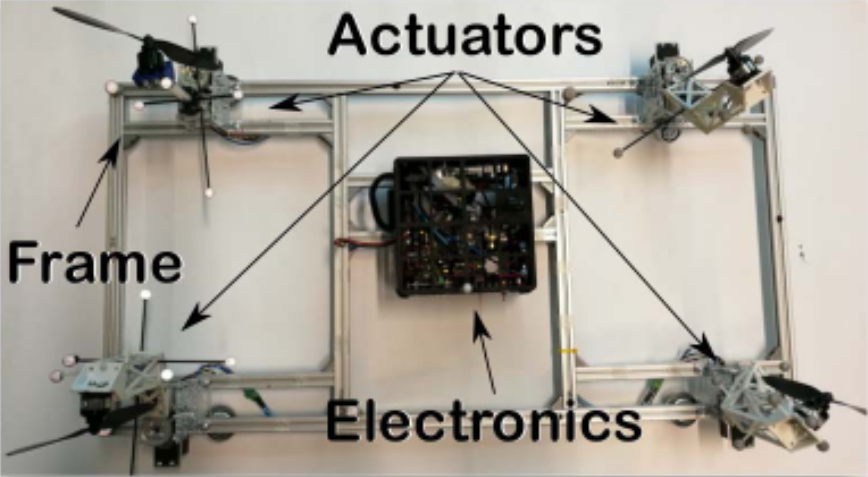
\includegraphics[width=5cm]{Images/rospo-paper}
    \caption{photo of the ROSPO prototype, courtesy of \cite{rospo}.}
    \label{fig:rospomech}
\end{figure}


The proposed idea is to use artificial neural networks trained offline on a dataset obtained by solving non-linear allocation problems; Khan et al. \cite{ANNallocator} reported promising results while solving allocation problem on an aerial vehicle, showing best regulation performance and lower evaluation time than common QP-based online solution.



This document will continue as follows: in Sec. \ref{sec:description} the ROSPO platform is described in more detail and its model is derived, Sec. \ref{sec:control} describes the control scheme that I used while Sec. \ref{sec:code} reports some implementation details. Later Sec. \ref{sec:results} reports some simulation results and finally conclusions are summarized in Sec. \ref{sec:conclusions}.
